\documentclass[twoside,twocolumn,10pt]{article}

% -----------------------------
% Packages
% -----------------------------
\usepackage{fancyhdr}
\usepackage{geometry}
\usepackage{abstract}
\usepackage{graphicx}
\usepackage{titlesec}
\usepackage{ragged2e}
\usepackage{amssymb}
\usepackage{parskip}
\usepackage{amsmath}
\usepackage{newtxtext}
\usepackage{booktabs}
\usepackage{array}
\usepackage{balance}
\usepackage[backend=bibtex,style=ieee]{biblatex}
\addbibresource{references.bib}
\usepackage[font=footnotesize,labelfont=bf,justification=raggedright,format=plain]{caption}
\usepackage{float}
\usepackage[hidelinks]{hyperref}
\usepackage{xcolor}

% -----------------------------
% Bibliography Heading
% -----------------------------
\defbibheading{bibliography}[\refname]{%
  \section{\MakeUppercase{REFERENCES}}}

% -----------------------------
% Custom Column Types
% -----------------------------
\newcolumntype{L}[1]{>{\raggedright\arraybackslash}p{#1}}
\newcolumntype{C}[1]{>{\centering\arraybackslash}p{#1}}
\newcolumntype{R}[1]{>{\raggedleft\arraybackslash}p{#1}}

% -----------------------------
% Caption Formatting
% -----------------------------
\captionsetup[table]{labelsep=period, justification=raggedright}
\captionsetup[figure]{labelsep=period, justification=raggedright}

% -----------------------------
% Page Geometry
% -----------------------------
\geometry{
    a4paper,
    left=0.8in,
    right=0.8in,
    top=1in,
    bottom=1in
}

\setlength{\columnsep}{15pt}
\setlength{\parindent}{0pt}
\setlength{\parskip}{0pt}
\hyphenpenalty=500
\exhyphenpenalty=500
\frenchspacing

% -----------------------------
% Abstract Formatting
% -----------------------------
\renewcommand{\abstractname}{\hspace{1.3em}\textbf{Abstract}}
\renewcommand{\abstractnamefont}{\normalfont\fontsize{10}{14}\bfseries\MakeUppercase}
\renewcommand{\absnamepos}{flushleft}
\renewcommand{\abstracttextfont}{\normalfont\fontsize{11}{13}\selectfont}

% -----------------------------
% Header / Footer Style
% -----------------------------
\setcounter{page}{1}
\pagestyle{fancy}
\fancyhf{}
\fancyhead[C]{\small AI-POWERED DATABASE-AS-A-SERVICE PLATFORM}
\fancyhead[CO]{\small Azmy et al. (2026)}
\fancyfoot[C]{\thepage}

% -----------------------------
% First Page Style
% -----------------------------
\fancypagestyle{firstpage}{
  \fancyhf{}
  \fancyhead[LO]{\small Volume X, Issue X, 2026}
 \fancyhead[RO]{\small LGU J. Comput. Sci. \& IT}
  \fancyfoot[L]{\footnotesize Received: DD Month YYYY; Revised: DD Month YYYY; Accepted: DD Month YYYY\\\textsuperscript{*}Corresponding Author: Hassan Hussein Azmy \textless hassanhusseinazmy@gmail.com\textgreater}
  \fancyfoot[R]{\footnotesize \textcopyright\ 2026 by the Author(s). Published by LGURJCSIT,\\ \hspace{0.5cm} under the CC-BY license}
  \renewcommand{\headrulewidth}{0.4pt}
  \renewcommand{\footrulewidth}{0.4pt}
}

% -----------------------------
% Title / Author
% -----------------------------
\title{\fontsize{16}{20}\selectfont\textbf{A UNIFIED AI-POWERED DATABASE-AS-A-SERVICE PLATFORM WITH MULTI-AGENT SCHEMA GENERATION AND TEXT-TO-SQL}}

\author{
    \fontsize{12}{14}\selectfont
    Hassan Hussein Azmy\textsuperscript{1*}, Abdullah Hany Ragab\textsuperscript{1}, Ali Mohamed Ali\textsuperscript{1},\\[0.5ex]
    Ahmed Bahy Youssef\textsuperscript{1}, Aya Mohammed Sayed\textsuperscript{1}\\[1ex]
    \fontsize{12}{14}\selectfont
    \textsuperscript{1}Department of Computer Systems Engineering, Benha University, Benha, Egypt
}

\date{}

% -----------------------------
% Section Formatting
% -----------------------------
\titleformat{\section}{\normalsize\bfseries\uppercase}{\thesection.}{1em}{}
\titleformat{\subsection}{\normalsize\bfseries\flushleft}{\thesubsection.}{1em}{}
\titleformat{\subsubsection}{\normalsize\bfseries\itshape\flushleft}{\thesubsubsection.}{1em}{}

% -----------------------------
% Document Start
% -----------------------------
\begin{document}

\twocolumn[
\begin{@twocolumnfalse}

\vspace{-0.7cm}
\noindent
\raggedright
{\fontsize{11}{13}\selectfont Original Article}
\hfill
{\fontsize{11}{13}\selectfont\footnotesize https://doi.org/xx.xxxx/xxxx}

\vspace{-0.5cm}

\maketitle
\thispagestyle{firstpage}

\section*{\hspace{-1.5mm}Abstract}
\fontsize{10}{12}\selectfont
\justifying
\noindent
Modern software development heavily relies on data, yet managing databases remains complex due to the coexistence of SQL and NoSQL systems, fragmented tools, and steep learning curves. Existing cloud-hosted database services simplify infrastructure but lack integrated development environments with intelligent assistance. This paper presents a unified, AI-powered Database-as-a-Service (DBaaS) platform that supports both PostgreSQL and NoSQL (MongoDB) databases within a single cloud-native interface. The platform features three core contributions: (1)~a Kubernetes-based multi-tenant provisioning engine with namespace-level isolation and operator-driven lifecycle management, (2)~a multi-agent AI service for automated schema generation from natural language descriptions using Retrieval-Augmented Generation (RAG) and deterministic normalization tools, and (3)~a multi-agent Text-to-SQL pipeline that translates natural language questions into executable SQL queries through schema selection, query decomposition, review, and iterative refinement. The schema generation service decomposes database design into specialized agents for conceptual, logical, and physical design stages, each verified through feedback loops. The Text-to-SQL service achieves 72.97\% execution accuracy on the BIRD benchmark. Provisioning latency averages 26.9 seconds on a local Kubernetes cluster, and idle tenants consume approximately 111~MiB of memory, enabling high-density multi-tenant deployments. The platform demonstrates that AI-assisted database management, cloud-native orchestration, and multi-engine support can be integrated into a practical, end-to-end development environment.

\vspace{0.3cm}
\noindent\textbf{Keywords:} Database-as-a-Service, multi-agent systems, schema generation, Text-to-SQL, Kubernetes, Retrieval-Augmented Generation, cloud-native, large language models


\vspace{0.8cm}
\end{@twocolumnfalse}
]

% -----------------------------
% Main Text
% -----------------------------
\section{Introduction}
\fontsize{11}{13}\selectfont

Databases form the backbone of modern software systems, supporting data storage, retrieval, analysis, and application logic. The increasing reliance on data-driven decision-making has elevated the need for efficient, scalable, and accessible database management systems, spanning relational databases (SQL) such as PostgreSQL and non-relational databases (NoSQL) such as MongoDB~\cite{codd1970}.

Database development, however, is often complex due to fragmented workflows involving multiple tools for schema design, data manipulation, query execution, and cloud hosting. While cloud-based services like AWS RDS~\cite{aws_rds_provisioning}, Supabase, Firebase, and MongoDB Atlas simplify infrastructure management, they do not provide fully integrated development environments, leaving inefficiencies and steep learning curves for developers~\cite{Comparison_of_dbaas_architectures, Database_as_a_service}.

Advances in artificial intelligence, particularly large language models (LLMs) and Retrieval-Augmented Generation (RAG)~\cite{lewis20}, offer opportunities for automated schema generation, optimized queries, and natural language interactions with databases. However, AI integration in existing database tools remains limited and disconnected from the database lifecycle~\cite{Text_to_SQL_Survey}.

This paper presents a unified, cloud-based Database-as-a-Service (DBaaS) platform that addresses these gaps. The platform supports PostgreSQL and MongoDB, combines visual schema design with AI-powered assistance, and provides an integrated environment for database provisioning, management, and querying. The key contributions are:

\begin{itemize}
    \item A \textbf{Kubernetes-based multi-tenant provisioning engine} with namespace-level isolation, operator-driven lifecycle management, and asynchronous state machine provisioning.
    \item A \textbf{multi-agent schema generation service} that translates natural language descriptions into normalized database schemas using RAG and deterministic normalization algorithms.
    \item A \textbf{multi-agent Text-to-SQL pipeline} that converts natural language questions into executable SQL through schema selection, query decomposition, review, and iterative refinement.
\end{itemize}


\section{Related Work}
\fontsize{11}{13}\selectfont

\subsection{Database-as-a-Service Platforms}

Database-as-a-Service (DBaaS) is a cloud service model in which providers manage the infrastructure, maintenance, and administration of databases on behalf of users~\cite{Database_as_a_service}. DBaaS architectures range from separate databases per tenant (virtual multi-tenancy) to shared-database, shared-schema designs (organic multi-tenancy), each trading isolation for resource efficiency~\cite{Comparison_of_dbaas_architectures}. Performance isolation remains a fundamental challenge, as multi-tenant environments must prevent ``noisy neighbor'' effects~\cite{Performance_Isolation_DBaaS, Solver_in_the_loop}.

Commercial platforms such as Amazon RDS, Azure SQL, Google Cloud SQL, MongoDB Atlas, and Supabase have established the standard for managed database hosting. However, these platforms exhibit several limitations relevant to this work: (a)~most support either SQL or NoSQL but not both; (b)~schema visualization and design tools are minimal or absent; (c)~AI-assisted features are limited; and (d)~vendor lock-in restricts portability.

% ------------------------------------------------------------------
% TABLE 1: Comparison of DBaaS platforms
% ------------------------------------------------------------------
\begin{table}[htbp]
\centering
\caption{Feature comparison of existing DBaaS platforms and the proposed system.}
\label{tab:dbaas_comparison}
\renewcommand{\arraystretch}{1.2}
\setlength{\tabcolsep}{4pt}
\resizebox{\columnwidth}{!}{
\begin{tabular}{l c c c c c}
\toprule
\textbf{Platform} & \textbf{SQL} & \textbf{NoSQL} & \textbf{Schema Viz.} & \textbf{Lock-in} & \textbf{AI} \\
\midrule
AWS RDS       & \checkmark & --         & Low      & High   & --         \\
DynamoDB      & --         & \checkmark & Low      & High   & --         \\
Google SQL    & \checkmark & --         & Low      & High   & --         \\
Firebase      & --         & \checkmark & --       & High   & --         \\
Azure SQL     & \checkmark & --         & Basic    & High   & --         \\
MongoDB Atlas & --         & \checkmark & Limited  & Low    & Limited    \\
Supabase      & \checkmark & --         & ERD      & Medium & Limited    \\
\midrule
\textbf{Proposed} & \checkmark & \checkmark & \textbf{Full} & \textbf{Low} & \textbf{Full} \\
\bottomrule
\end{tabular}
}
\end{table}

\subsection{AI Agents and Multi-Agent Systems}

Recent advances in LLMs have enabled the development of AI agents---autonomous systems that perceive their environment, reason about tasks, and take actions~\cite{AI_Agents_Evolution}. Multi-agent architectures extend this paradigm by decomposing complex problems across specialized agents, each responsible for a distinct subtask, coordinated through structured communication protocols~\cite{autogen, yao22}. The ReAct framework~\cite{yao22} demonstrated the effectiveness of interleaving reasoning and tool use, while AutoGen~\cite{autogen} introduced a flexible multi-agent conversation framework for orchestrating LLM-based workflows.

\subsection{Text-to-SQL}

Text-to-SQL aims to translate natural language questions into executable SQL queries. Multi-agent approaches such as MAC-SQL~\cite{Multi_Agent_Text_to_SQL} decompose the problem into schema selection, query generation, and refinement stages, achieving state-of-the-art results on benchmarks like Spider~\cite{yu2018spider} and BIRD. The integration of RAG with structured prompting has further improved accuracy by grounding model outputs in actual schema information~\cite{Text_to_SQL_Survey, Optimizing_text_to_SQL}.

\subsection{AI-Assisted Schema Design}

Traditional database design follows a well-established lifecycle: requirements analysis, conceptual design (ER modeling)~\cite{chen1976}, logical design (normalization to 3NF)~\cite{bernstein1976}, and physical design. Recent work has explored using LLMs to automate parts of this pipeline, but most approaches treat schema generation as a single-pass text generation problem, producing outputs that may violate normalization rules or contain inconsistent keys. Our work addresses this by combining LLM reasoning with deterministic normalization algorithms within a multi-agent feedback loop.


\section{System Architecture}
\fontsize{11}{13}\selectfont

The platform follows a control-plane/data-plane separation. The control plane handles user authentication, metadata management, and infrastructure orchestration. The data plane encapsulates the provisioned tenant database instances, connection routing, and query execution paths.

% ------------------------------------------------------------------
% FIGURE PLACEHOLDER: High-Level Architecture
% ------------------------------------------------------------------
\begin{figure*}[t]
\centering
% TODO: Replace with your system architecture diagram
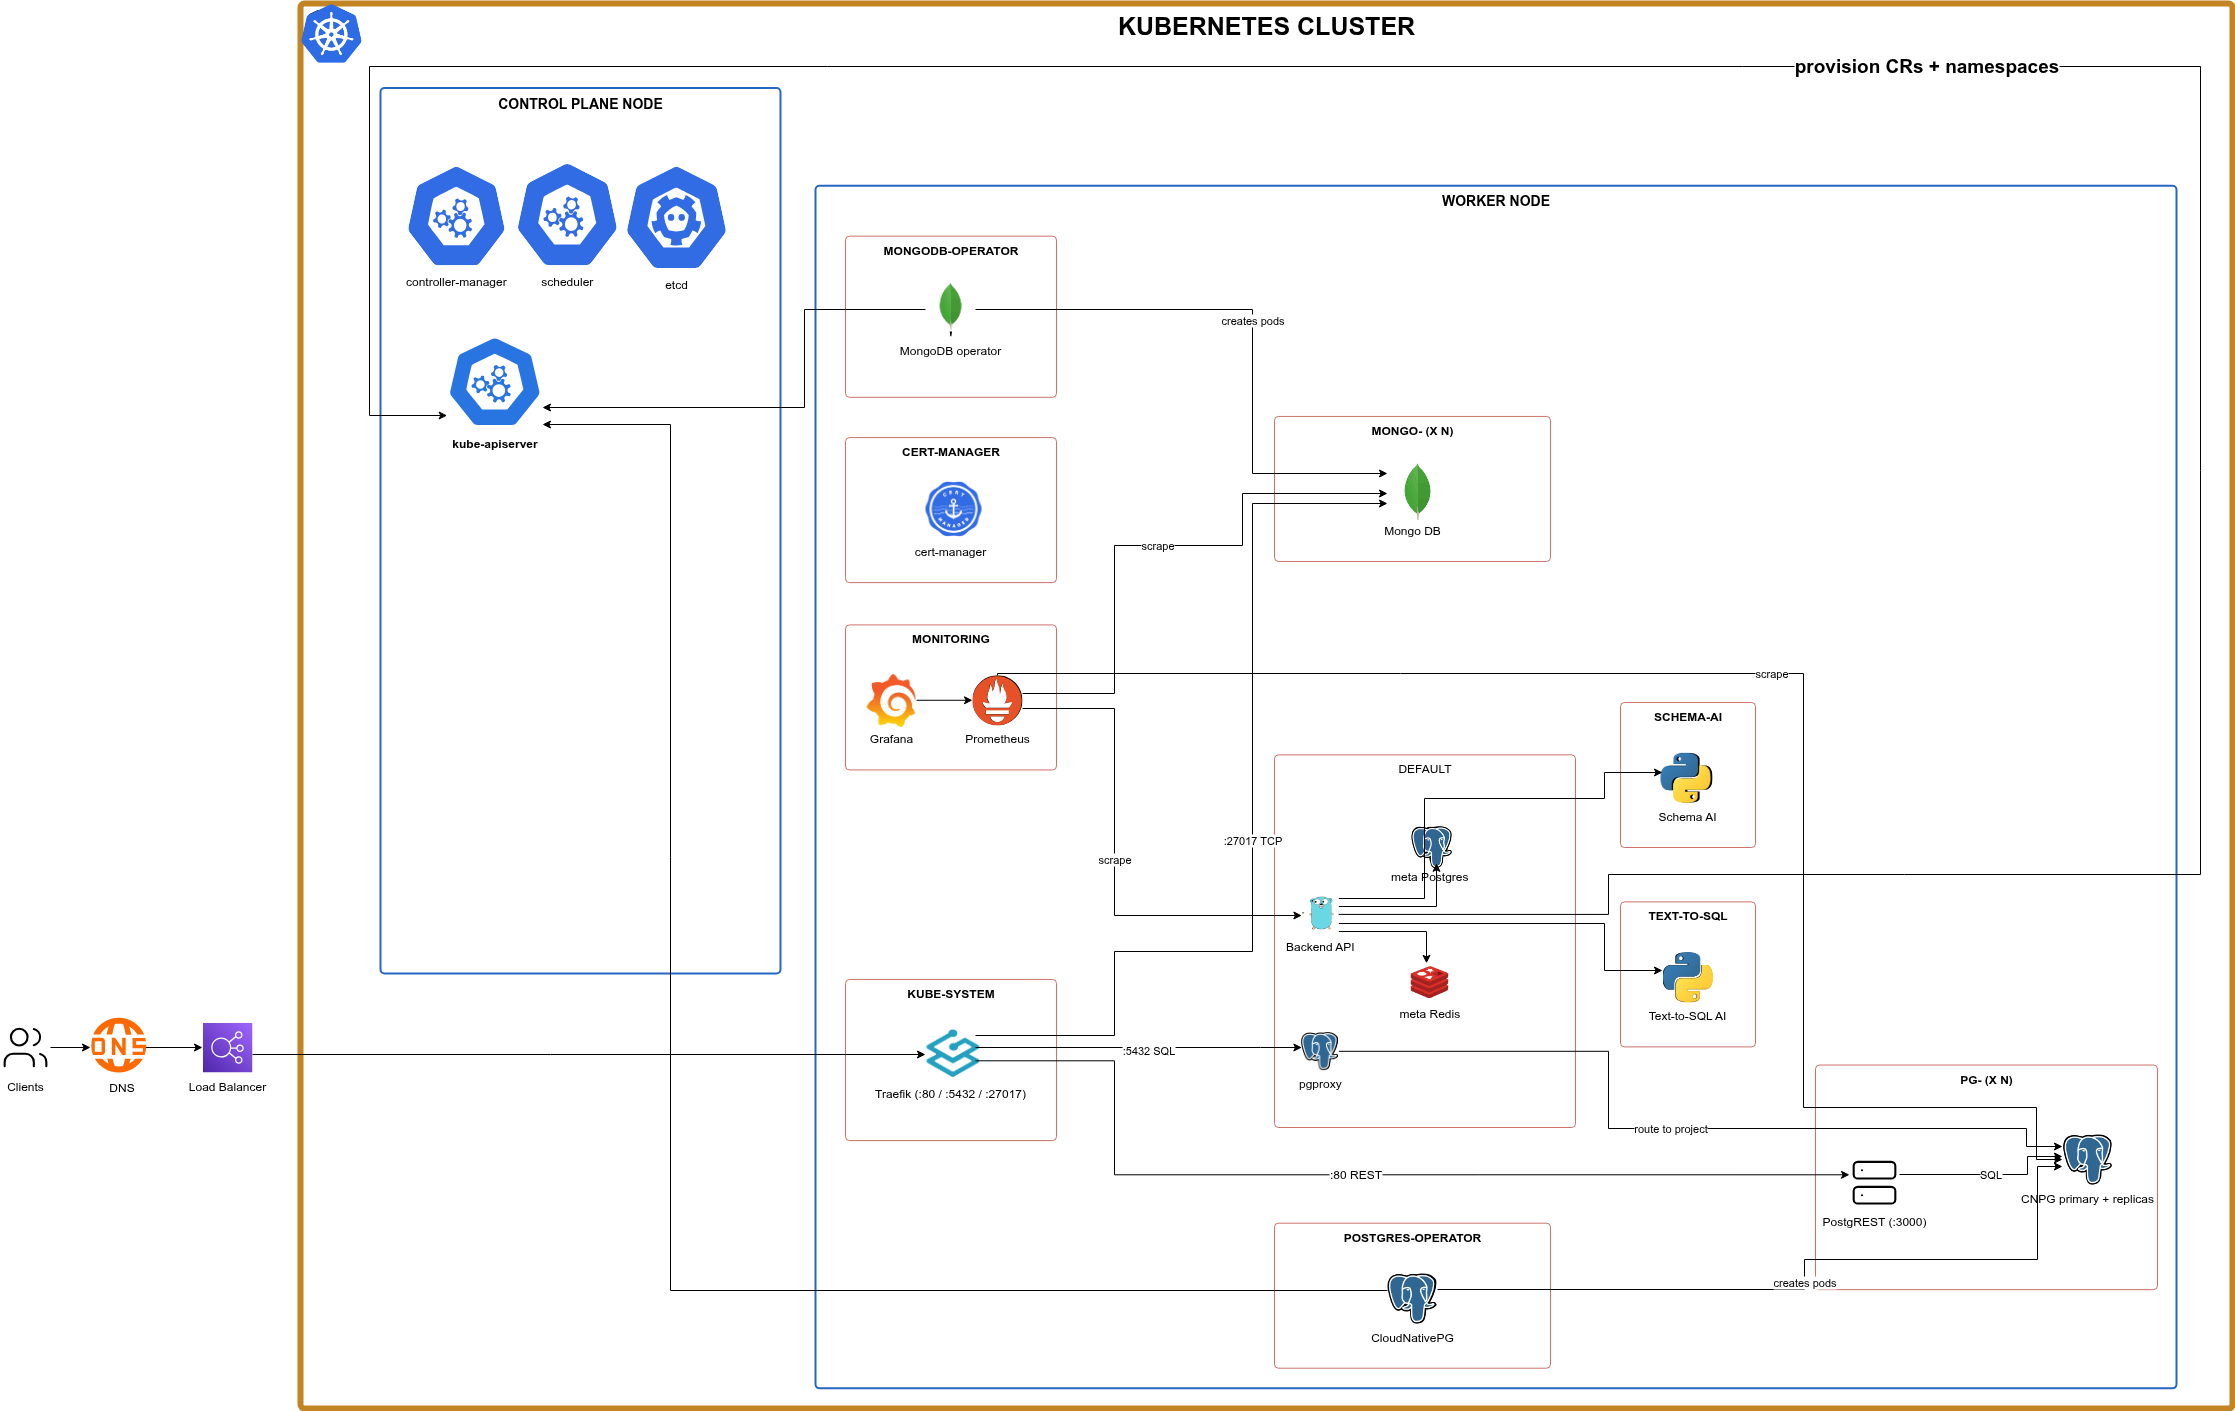
\includegraphics[width=0.82\textwidth]{architecture.png}
\caption{High-level system architecture showing the control plane, data plane, AI services, and client interfaces.}
\label{fig:architecture}
\end{figure*}

\subsection{Control Plane}

The control plane exposes a REST API (built in Go with the Gin framework), manages platform metadata in a dedicated PostgreSQL instance, and uses Redis for caching and asynchronous task queuing. Key components include:

\begin{itemize}
    \item \textbf{Ingress and API Gateway (Traefik):} Handles TLS termination, HTTP routing, and TCP/SNI passthrough for direct database connections.
    \item \textbf{Orchestration Worker:} Consumes provisioning tasks from a message queue and interacts with the Kubernetes API to create tenant namespaces, inject secrets, and submit Custom Resources to database operators.
    \item \textbf{Kubernetes Operators:} CloudNativePG~\cite{cloudnativepg} and the MongoDB Community Operator~\cite{mongodb_operator} declaratively manage database cluster lifecycles.
\end{itemize}

\subsection{Asynchronous Provisioning State Machine}

Database provisioning is modeled as an asynchronous state machine to avoid blocking the API. When a user requests a new database, the system validates the request, registers the project with a \textit{creating} status, and enqueues a provisioning task. A background worker then creates an isolated Kubernetes namespace, injects cryptographic secrets, and submits Custom Resources. The worker polls for readiness, transitioning the project to \textit{running} on success or \textit{failed} on timeout.

\subsection{Multi-Tenant Isolation}

Each tenant project is provisioned into a dedicated Kubernetes namespace (e.g., \texttt{pg-<uuid>} or \texttt{mongo-<uuid>}), enclosing the database cluster, Secrets, Services, and engine-specific sidecars. This namespace-level isolation ensures that cross-tenant data access is structurally impossible at the network layer. Resource tiers enforce CPU, memory, and storage limits via Kubernetes resource quotas.

\subsection{Data Plane Routing}

For direct relational database access, a dedicated TLS routing proxy (PGProxy) inspects the SNI extension in the TLS \texttt{ClientHello} packet to extract the project identifier and routes the TCP stream to the appropriate namespace without terminating encryption. This preserves end-to-end TLS between the client and the tenant database.

\subsection{Security Architecture}

The platform operates under zero-trust assumptions. Tenant credentials are generated during provisioning and stored only in Kubernetes Secrets within the tenant's namespace---the control plane meta-database never stores raw connection strings. Role-Based Access Control (RBAC) constrains the orchestrator's Kubernetes permissions to the minimum required. AI-generated queries are treated as untrusted input and pass through a query safety validator that blocks destructive operations.


\section{AI-Assisted Schema Generation}
\fontsize{11}{13}\selectfont

The schema generation service takes a natural language description of an application and produces a relational database design: an entity-relationship model, normalized relations in third normal form (3NF), executable PostgreSQL DDL, and a structured report.

\subsection{Multi-Agent Workflow}

Rather than relying on a single LLM call, the service decomposes schema generation into specialized agents that mirror the classical database design lifecycle. Table~\ref{tab:schema_agents} lists the agent roles.

% ------------------------------------------------------------------
% TABLE 2: Schema Generation Agents
% ------------------------------------------------------------------
\begin{table}[htbp]
\centering
\caption{Agent roles in the schema generation service.}
\label{tab:schema_agents}
\renewcommand{\arraystretch}{1.2}
\setlength{\tabcolsep}{4pt}
\resizebox{\columnwidth}{!}{
\begin{tabular}{l p{5cm}}
\toprule
\textbf{Agent} & \textbf{Responsibility} \\
\midrule
Manager & Reads the requirement, fills in implied needs, and decides final acceptance. \\
Conceptual Designer & Extracts entities, attributes, relationships, and cardinalities into an ER model. \\
Conceptual Reviewer & Validates the conceptual model against design rules and requests revisions. \\
Logical Designer & Converts the approved model into normalized relations using deterministic tools. \\
QA & Generates representative test cases from the requirement without seeing the schema. \\
Execution & Judges whether the schema satisfies the test cases. \\
Physical Designer & Infers PostgreSQL types, writes DDL with indexes, and validates against a real database. \\
Report & Compiles all stages into a structured document. \\
\bottomrule
\end{tabular}
}
\end{table}

\subsection{Coordination and Feedback Loops}

Two feedback loops provide self-correcting behavior. The \textit{inner loop} iterates between the conceptual designer and reviewer until the reviewer signals approval, applying fixed validation procedures. The \textit{outer loop} runs QA-generated test cases against the schema; failures are routed back to the responsible design stage. Both loops are bounded by a maximum iteration count.

\subsection{Deterministic Normalization Tools}

The most error-prone parts of logical design---key discovery and normalization---use deterministic algorithms rather than free LLM generation. The logical designer declares functional dependencies and invokes two tools: (1)~a candidate key finder using attribute-closure search under Armstrong's axioms, and (2)~a 3NF decomposition algorithm that detects partial and transitive dependencies~\cite{bernstein1976}. This ensures normalization correctness by construction.

\subsection{Domain-Aware Retrieval}

The service includes a curated knowledge base covering six application domains (healthcare, e-commerce, finance, education, logistics, and human resources). When a requirement arrives, the service infers its domain and makes relevant entity patterns, relationship conventions, and type mappings available to the agents via retrieval-augmented tools. Embeddings use the \texttt{all-MiniLM-L6-v2} sentence transformer with cosine similarity search.

% ------------------------------------------------------------------
% FIGURE PLACEHOLDER: Schema Generation Architecture
% ------------------------------------------------------------------
\begin{figure}[htbp]
\centering
\fbox{\begin{minipage}{0.92\columnwidth}
\centering
\vspace{2.5cm}
\textbf{\large [TEXT-TO-SCHEMA ARCHITECTURE IMAGE]}

\smallskip
\small Replace this placeholder with the multi-agent schema generation architecture diagram.
\vspace{2.5cm}
\end{minipage}}
\caption{Multi-agent schema generation pipeline showing the inner conceptual review loop and outer validation loop.}
\label{fig:schema_pipeline}
\end{figure}


\section{Text-to-SQL Service}
\fontsize{11}{13}\selectfont

The Text-to-SQL service translates natural language questions into executable SQL queries through a four-agent pipeline.

\subsection{Agent Pipeline}

\begin{enumerate}
    \item \textbf{Selector:} Identifies relevant tables and columns from the full database schema using semantic matching, reducing context size for downstream agents.
    \item \textbf{Decomposer:} Breaks complex questions into sub-questions using chain-of-thought prompting, generating intermediate SQL fragments and a final combined query.
    \item \textbf{SQL Reviewer:} Validates syntax, schema consistency, type compatibility, and logical coherence. Outputs a structured pass/fail report.
    \item \textbf{Refiner:} Addresses issues identified by the reviewer, corrects logical errors, and ensures alignment with user intent. Operates in an iterative loop with the reviewer.
\end{enumerate}

Each agent uses carefully engineered prompts combining system instructions, structured schema context, and few-shot examples. The Selector and Reviewer use deterministic decoding (temperature~=~0), while the Decomposer allows modest stochasticity for creative reasoning.

% ------------------------------------------------------------------
% FIGURE PLACEHOLDER: Text-to-SQL Pipeline
% ------------------------------------------------------------------
\begin{figure*}[t]
\centering
\fbox{\begin{minipage}{0.70\textwidth}
\centering
\vspace{0.2cm}
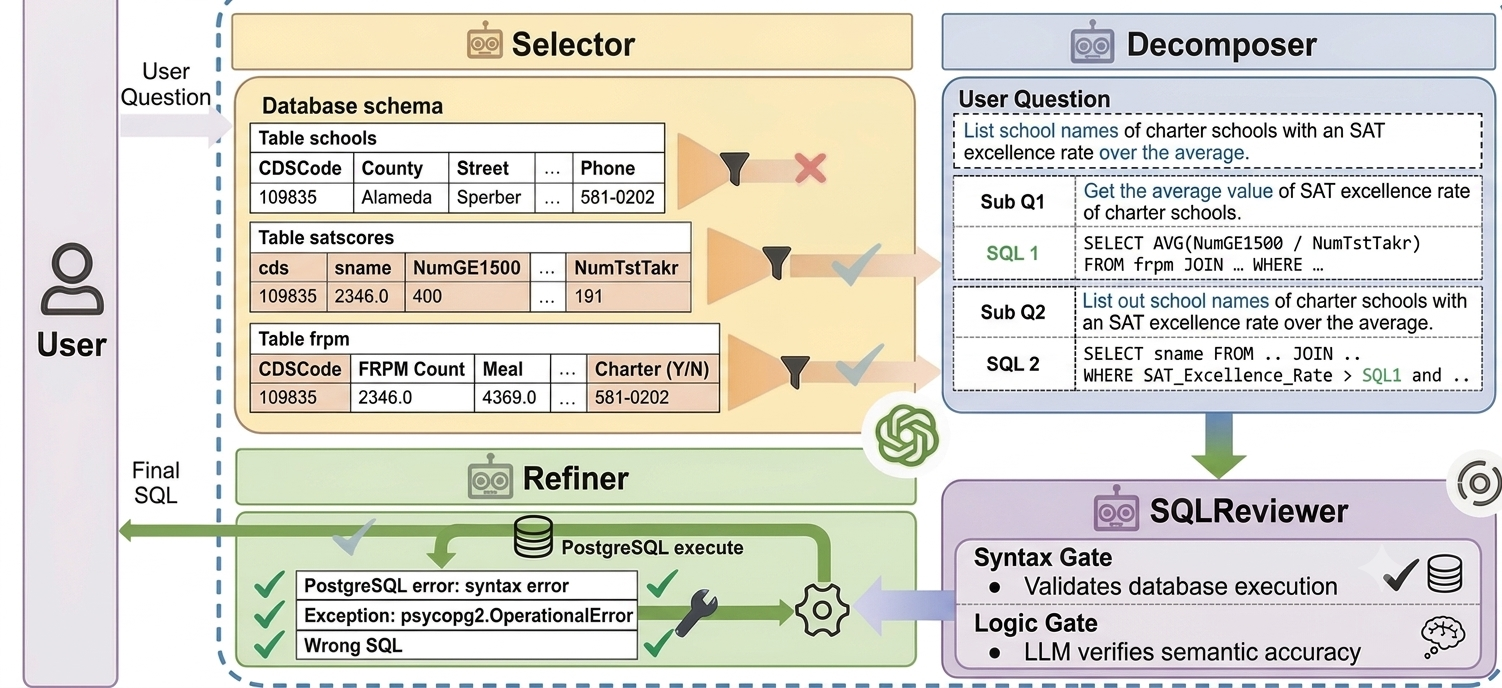
\includegraphics[width=0.95\textwidth]{text2SQL.png}
\vspace{0.2cm}
\end{minipage}}
\caption{Text-to-SQL multi-agent pipeline: Selector, Decomposer, Reviewer, and Refiner stages.}
\label{fig:text2sql_pipeline}
\end{figure*}

\section{Evaluation}
\fontsize{11}{13}\selectfont

\subsection{Text-to-SQL Performance}

The Text-to-SQL service was evaluated on a subset of the BIRD benchmark (\texttt{mini\_dev}), migrated from SQLite to PostgreSQL. Two metrics are reported: Execution Accuracy (EX), measuring the percentage of queries producing correct results, and Valid Efficiency Score (VES), measuring the execution efficiency of correct queries relative to gold-standard queries.

% ------------------------------------------------------------------
% TABLE 3: Text-to-SQL Results
% ------------------------------------------------------------------
\begin{table}[htbp]
\centering
\caption{Text-to-SQL performance on the BIRD \texttt{mini\_dev} benchmark by query complexity.}
\label{tab:text2sql_results}
\renewcommand{\arraystretch}{1.2}
\setlength{\tabcolsep}{3pt}
\resizebox{\columnwidth}{!}{
\begin{tabular}{l c c c c}
\toprule
\textbf{Metric} & \textbf{Simple} & \textbf{Moderate} & \textbf{Challenging} & \textbf{Total} \\
\midrule
Query Count      & 62    & 47     & 39     & 148  \\
Passed Queries   & 50    & 31     & 27     & 108  \\
Mismatches       & 12    & 16     & 12     & 39   \\
EX Accuracy (\%) & 80.65 & 65.96  & 69.23  & 72.97 \\
VES Score (\%)   & 83.26 & 64.52  & 73.73  & 74.80 \\
\bottomrule
\end{tabular}
}
\end{table}

The pipeline achieves 72.97\% overall execution accuracy. Performance is highest on simple queries (80.65\%) and shows a recovery on challenging queries (69.23\% vs.\ 65.96\% for moderate), suggesting that the multi-agent pipeline's explicit decomposition and error correction mechanisms are particularly effective for complex queries.

\subsection{Provisioning Latency}

Five free-tier PostgreSQL projects were provisioned sequentially on a local k3d cluster (K3s, single node). Time-to-\textit{running} includes namespace creation, Secret injection, CloudNativePG reconciliation, PVC binding, pod startup, and PostgREST sidecar deployment.

% ------------------------------------------------------------------
% TABLE 4: Provisioning Latency
% ------------------------------------------------------------------
\begin{table}[htbp]
\centering
\caption{PostgreSQL provisioning latency on a local k3d cluster (free tier).}
\label{tab:provisioning}
\renewcommand{\arraystretch}{1.2}
\setlength{\tabcolsep}{5pt}
\begin{tabular}{c c c c c c c}
\toprule
\textbf{Run} & 1 & 2 & 3 & 4 & 5 & \textbf{Mean} \\
\midrule
Seconds & 20.4 & 26.5 & 26.4 & 30.5 & 30.5 & 26.9 \\
\bottomrule
\end{tabular}
\end{table}

The mean provisioning latency is 26.9~seconds, substantially faster than managed cloud services (which typically require several minutes)~\cite{aws_rds_provisioning}. Variation across runs reflects Kubernetes scheduling and storage binding jitter.

\subsection{Resource Footprint}

An idle free-tier PostgreSQL project consumes approximately 86~MiB (CloudNativePG pod) + 25~MiB (PostgREST sidecar) = 111~MiB of RSS. On a 16~GiB worker node, this permits approximately 120--130 idle projects, demonstrating viable multi-tenant density for the containerized isolation model.

\subsection{PGProxy Routing}

Internal benchmarking using \texttt{pgbench} (TPC-B, single client, 10-second duration) reported 0.834~ms average transaction latency and approximately 1,199~TPS. PGProxy performs TLS passthrough without termination, so the dominant costs are PostgreSQL execution and network RTT rather than proxy inspection overhead.


\section{Discussion}
\fontsize{11}{13}\selectfont

\subsection{Contributions}

The platform's primary contribution is not a single model or endpoint, but the \textit{orchestration of several services into a practical, integrated platform}. By combining Kubernetes-based provisioning, multi-agent AI services, and a unified API, the system reduces manual database setup effort while providing intelligent assistance throughout the development lifecycle.

The multi-agent schema generation approach offers specific advantages over single-pass LLM generation: (a)~errors are caught at the stage where they are introduced through feedback loops, (b)~normalization is guaranteed through deterministic algorithms rather than model generation, and (c)~domain-specific knowledge improves design quality through targeted RAG.

\subsection{Limitations}

Several limitations should be acknowledged:

\begin{itemize}
    \item \textbf{AI reliability:} The AI services remain sensitive to prompt quality, schema size, and query complexity. Even syntactically valid outputs can be semantically incorrect.
    \item \textbf{Text-to-SQL accuracy:} The 72.97\% execution accuracy, while competitive, means approximately 27\% of natural language queries are not correctly translated, requiring user verification.
    \item \textbf{Evaluation scope:} Performance metrics were collected on a local single-node k3d cluster; production cloud environments may exhibit different characteristics.
    \item \textbf{Token budget:} Schemas exceeding LLM context limits cannot be fully represented, requiring manual schema curation for very large databases.
    \item \textbf{Latency:} Multi-agent generation introduces 2--8 seconds of latency per query, unsuitable for real-time interactive dashboards.
\end{itemize}

% ------------------------------------------------------------------
% PLACEHOLDER: Additional figures/tables you may want to add
% ------------------------------------------------------------------

% TODO [OPTIONAL]: Figure - Screenshot of the platform UI showing the schema builder
% \begin{figure}[htbp]
% \centering
% \includegraphics[width=\columnwidth]{ui_screenshot.png}
% \caption{Platform UI: visual schema builder interface.}
% \label{fig:ui_screenshot}
% \end{figure}

% TODO [OPTIONAL]: Figure - Screenshot of the Text-to-SQL conversational interface
% \begin{figure}[htbp]
% \centering
% \includegraphics[width=\columnwidth]{text2sql_ui.png}
% \caption{Text-to-SQL conversational interface.}
% \label{fig:text2sql_ui}
% \end{figure}

% TODO [OPTIONAL]: Table - RAG domain coverage and retrieval performance
% TODO [OPTIONAL]: Table - Comparison of schema generation quality metrics across models


\section{Conclusion and Future Work}
\fontsize{11}{13}\selectfont

This paper presented a unified, AI-powered Database-as-a-Service platform that integrates multi-tenant database provisioning, multi-agent schema generation, and Text-to-SQL capabilities into a single cloud-native environment. The platform supports both PostgreSQL and MongoDB, employs Kubernetes operators for declarative lifecycle management, and uses Retrieval-Augmented Generation to enhance AI-assisted database design.

The schema generation service demonstrates that decomposing database design into specialized agents with deterministic normalization tools and feedback loops produces more reliable schemas than single-pass generation. The Text-to-SQL pipeline achieves 72.97\% execution accuracy on the BIRD benchmark through a four-agent architecture with iterative refinement. The provisioning engine delivers databases in under 30 seconds with approximately 111~MiB per-tenant overhead, enabling practical multi-tenant density.

Future work includes: (1)~unified workflow automation connecting schema generation directly to provisioning and query generation, (2)~support for multi-region and multi-cloud deployments, (3)~fine-tuning smaller domain-specific models to reduce cost and latency, (4)~distributed log tracing across microservices, (5)~stronger end-to-end integration testing on live Kubernetes clusters, and (6)~interactive user feedback loops to improve AI-generated outputs over time.


\vspace{0.5cm}

\small
\textbf{Conflict of Interest:} The authors declare no conflict of interest.

\textbf{Author Contributions:} H.H. Azmy designed and implemented the backend system, provisioning engine, and PGProxy. A.H. Ragab implemented the Text-to-SQL service. A.M. Ali developed the AI-assisted schema generation service. A.B. Youssef contributed to deployment and infrastructure. A.M. Sayed developed the frontend interface. All authors contributed to testing and manuscript preparation.

\textbf{Funding:} This research received no external funding.

\textbf{Ethical Statement:} This study follows ethical and academic integrity guidelines.

\textbf{Supervisor:} Dr. Rania Ramadan Abdel-Dayem and Eng. Mustafa Shokry, Department of Computer Systems Engineering, Faculty of Engineering, Benha University.

\balance
\fontsize{11}{13}\selectfont
\printbibliography

\end{document}